\begin{marginfigure}

\includegraphics[width=\textwidth]{ch02/figures/pylogo.jpg}
\caption{The Python programming language is an open source language that is increasingly popular for data science and signal processing.}
\end{marginfigure}

\newthought{We'll demonstrate various signal processing topics using
  programming} examples. Why \index{Python}{Python} and not some other
language? Here are three justifications:
\begin{itemize}
\item It is free for everyone to use,
\item there are a wide range of efficient numerical libraries available,
\item and Python is nowadays the language that students are most familiar with.
%\item Python has a built-in complex data type, both in single precision and double precision
\end{itemize}

\begin{marginfigure}
\begin{center}

\includegraphics[width=0.5\textwidth]{ch02/figures/numpylogo.png}
\end{center}
\caption{The NumPy package implements a large collection of numerical routines that can be used for signal processing.}
\end{marginfigure}

All the programming examples we'll show in these lecture notes will
support Python 3. We will restrict ourselves to a bare minimum number
of library dependencies. The main libraries you will need are:
\verb|numpy|, \verb|scipy|, and \verb|matplotlib|. These should be
readily available for nearly every operating system.

\begin{marginfigure}
\begin{center}

\includegraphics[width=0.68\textwidth]{ch02/figures/scipy.jpg}
\end{center}
\caption{The Scipy package contains a number of signal processing routines for Python.}
\end{marginfigure}

If you don't know how to obtain Python for your computer, you could
try out the Anaconda distribution of Python. It provides a relatively
complete set of the most commonly used Python modules. You can obtain
this distribution by visiting the anaconda web page:
\url{http://anaconda.org} and downloading the installer for your
platform.

The Anaconda package manager will allow you to install Numpy, Scipy,
and Matplotlib. Anaconda also comes with a Python development
environment as well. If you don't have your mind set on a specific
programming editor yet, you could try out the Spyder development
environment that comes with Anaconda.

\begin{marginfigure}

\includegraphics[width=\textwidth]{ch02/figures/matplotlib.png}
\caption{Matplotlib implements a basic plotting routines for Python.}
\end{marginfigure}

If you are using Linux, like I am most of the time, it is
probably easiest to just obtain Python using the system package
manager. On Ubuntu, you would install the necessary packages with the following command:
\begin{lstlisting}[language=sh,caption=Installing Python on Ubuntu Linux,label=lst:linuxinstall]
sudo apt-get install python3 python3-numpy python3-scipy python3-imageio python3-matplotlib ipython3
\end{lstlisting}

\begin{marginfigure}[3cm]

\includegraphics[width=0.68\textwidth]{ch02/figures/analogo.jpg}
\caption{The Anaconda distribution is currently one of the most
  popular distributions of the Python programming language, offering
  nearly all existing open source modules.}
\end{marginfigure}

After installing Python and the required modules, I recommend that you
write a short test program to make sure that all the modules are
installed correctly. To test your Python installation, open up your
programming editor and write a small Python program:
\lstinputlisting[language=Python,caption={\texttt{001\_hello\_world/hello.py}},label=lst:pythonhw]{code/001_hello_world/hello.py}
This test program prints out the standard hello world message, and
uses NumPy and SciPy to print the approximate value of $\pi$. The program then
plots a complex sinusoidal signal with the help of NumPy and
Matplotlib.  If you can run this program without getting any errors,
you are all set. The output should look something like this:

\begin{figure}
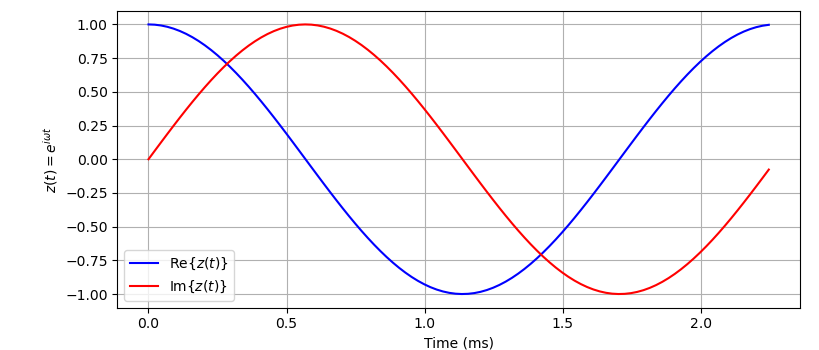
\includegraphics[width=\textwidth]{ch02/figures/testscreen1.png}
\caption{Output of the \texttt{hello.py} test program.}
\end{figure}

\newthought{Code examples} that are spread throughout these lecture
notes can be downloaded from GitHub:
\url{https://github.com/jvierine/signal_processing.git}. The easiest
way to access the code is to just visit this page with your web
browser. In order to download the source code for the examples in
these lecture notes, you can also use git on the command line:
\begin{lstlisting}[language=sh,caption=Obtaining the source code for the programming examples with git,label=lst:download]
git clone https://github.com/jvierine/signal_processing
\end{lstlisting}
If you are using Anaconda, you will have to install git (if you don't
have it already) by typing in
\begin{lstlisting}[language=sh,caption=Obtaining the source code for the programming examples with git,label=lst:download]
  conda install -c anaconda git
\end{lstlisting}
Then you can proceed with the command shown above. 

\begin{marginfigure}

\includegraphics[width=0.68\textwidth]{ch02/figures/gitlogo.png}
\caption{Program examples from these lecture notes are available on GitHub.}
\end{marginfigure}
